Найдем зависимость средних диаметров для желтых пар колец Na от разности диаметров
для колец одного порядка. Построим график $\overline{d} = F(1/\Delta d)$ и по
углу его наклона рассчитаем разность длин волн $\Delta \lambda$ для желтой пары
линий ртути

\import{src/}{hg_yellow_circ.tex}

\begin{figure}
  \center{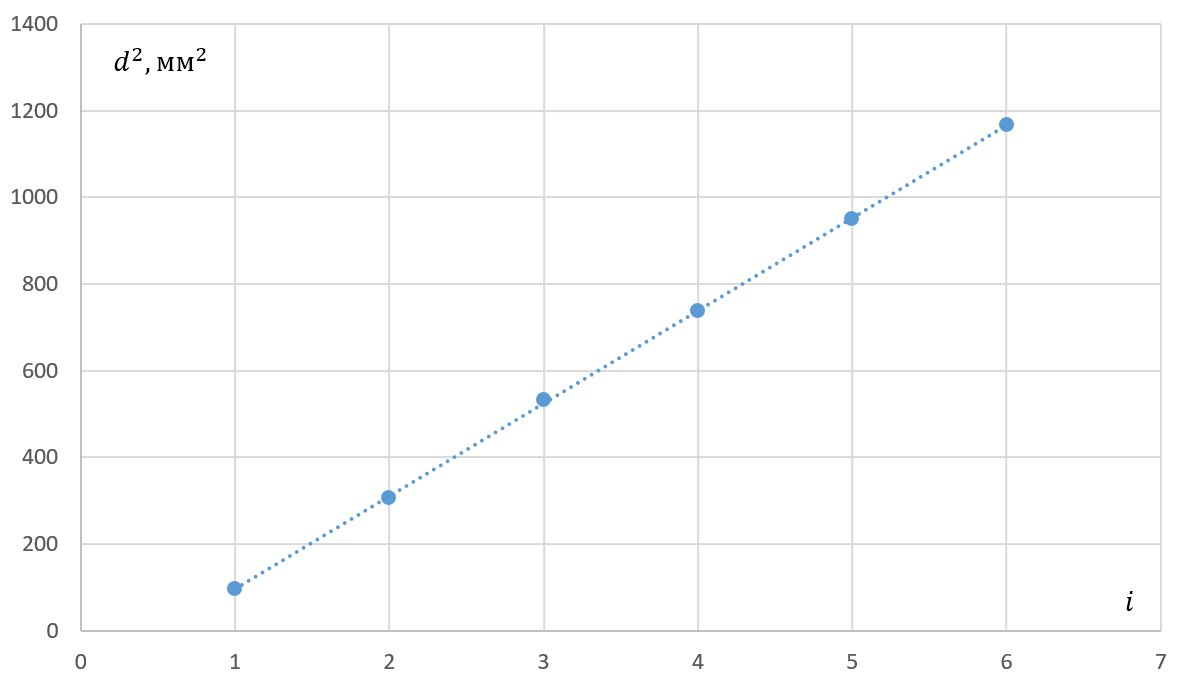
\includegraphics[width=\linewidth]{graph_hg_d_from_i.png}}
  \caption{$\overline{d} = F(1/\Delta d)$}
  \label{img::avg_diam_hg}
\end{figure}

\hfill \break

Аналогичную процедуру проведем для натрия.
\begin{table}
  \begin{center}
    \import{src/}{na.tex}
  \end{center}
  \caption{Измерение диаметров желтых колец натриевой лампы}
\end{table}

\begin{figure}
  \center{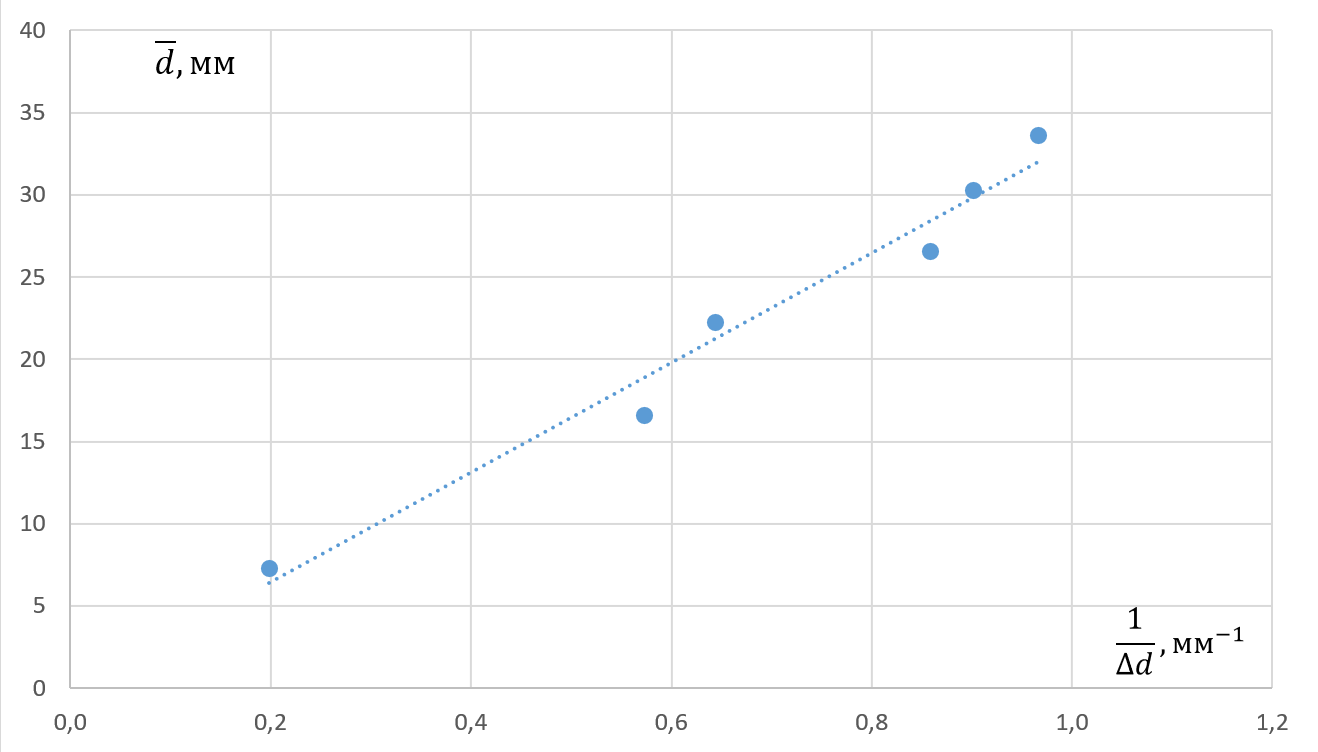
\includegraphics[width=\linewidth]{graph_na_avd_delta.png}}
  \caption{$\overline{d} = F(1/\Delta d)$}
  \label{img::avg_diam_na}
\end{figure}


